\chapter{Platform}
\label{chp:Platform}

\section{Implementation}
\label{sec:Implementation}
A device has been made to generate, receive and analyse flashes. The system architecture can be seen in figure \ref{fig:systemOveriew}. Each component their interfaces will be discussed briefly. Schematics of the electronics used for building the system can be found in appendix \ref{app_schematics}.

\begin{figure}[!h]
	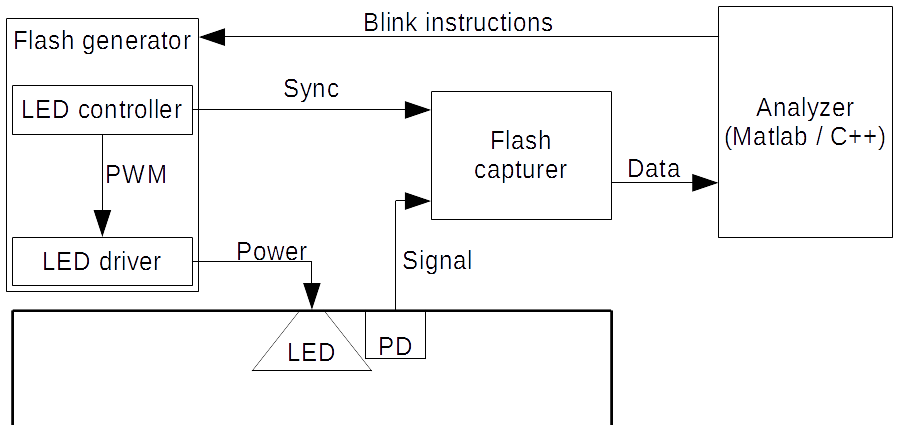
\includegraphics[width=\textwidth]{pics/systemOverview.png}
	\caption{System architecture of the flash generator/analyser}
	\label{fig:systemOveriew}
\end{figure}

\subsection{Flash generator}
The flash generator is a device able to control a LED with high precision. It is able to set the period $T$, and the t-on time $T_{on}$. $T$ Controls the frequency of the flashes and $t_{on}$ controls the amount of time the LED is turned on. Both parameters can be set with a resolution of $10\mu s$ resulting in a precisely controlled flash.

\begin{equation}
\label{eq:1/f=T}
T=\frac{1}{f}
\qquad
Duty cycle=\frac{T_{on}}{T} * 100\%
\end{equation}

\begin{figure}[!h]
	\centering
	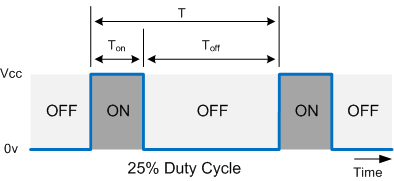
\includegraphics[]{pics/DutyCycle.png}
	\caption{Visualization of how $T$ and $T_{on}$ determine the duty cycle and frequency of the flash generator}
	\label{fig:DutyCycle}
\end{figure}

\subsection{Reflection receiver}
The job of the receiver is to sample values while the light is being turned on and off, to then analyse the full flash and extract it's features. 


\subsection{Analyser}
The analyser will receive samples from the reflection receiver and is ran on a PC in the form of either a C/C++ program (real-time) or as a matlab script (post-time).

If the receiver sends raw flashes to the anlyser it can be used to analyse this flash. This is used in section \ref{sec:Flash_characteristics}. If the receiver send compressed flashes, the analyser is able to analyse consecutive flashes. This mode will be used in chapter \ref{sec:Algorithm}.
